\documentclass{article}
\usepackage{amssymb,lineno}
\modulolinenumbers[5]
\usepackage{color}
\usepackage[colorlinks,linkcolor=black,hyperindex,CJKbookmarks,dvipdfm]{hyperref}
\usepackage{tikz}
\usetikzlibrary{shapes.geometric}
\usetikzlibrary{arrows.meta}
\usepackage{graphics,graphicx}
\usepackage{mathrsfs}
\usepackage{amsmath,bm}
\usepackage{subfigure}
\usepackage{booktabs}
\usepackage{amsthm}
\usepackage{subfigure}
\usepackage{listings}
\usepackage{setspace}
\usepackage[margin=2.5cm]{geometry}
\usetikzlibrary{shapes.geometric, arrows,matrix,positioning,calc}
\intextsep=8pt plus 3pt minus 1pt
\tikzstyle{startstop} = [rectangle, rounded corners, minimum width=2cm, minimum height=1cm,text centered, draw=black, fill=red!30]
\tikzstyle{process} = [rectangle, minimum width=4cm, minimum height=4cm, text centered, draw=black, fill=orange!30]
\tikzstyle{decision} = [diamond, minimum width=2cm, minimum height=1cm, text centered, draw=black, fill=green!30]
\theoremstyle{plain}\newtheorem{definition}{\sc{Definition}}
\theoremstyle{defination}\newtheorem{example}{Example}[section]
\definecolor{ColorMark}{rgb}{1,1,1}
\numberwithin{equation}{section}
\numberwithin{table}{section}
\graphicspath{{picture/}} 
\bibliographystyle{elsarticle-num}

\begin{document}

\title{A new HLLC Riemann solver to resolve both elactic and plastic waves}
\author{Li Liu$^1$,Junbo Cheng $^{1,*}$, Yiqing Shen$^2$}
%\cortext[mycorrespondingauthor]{
%Correspondence to: Yiqing Shen, LHD, Institute of Mechanics, Chinese Academy of Sciences, Beijing 100190, China. E-mail: yqshen@imech.ac.cn}
%\address{$^1$LHD, Institute of Mechanics, Chinese Academy of Sciences, Beijing 100190, China}
%\address{$^2$School of Engineering Science, University of Chinese Academy of Sciences, Beijing 100049, China}
%{
%\begin{abstract}
%In this paper, we construct a new numerical method to solve the reactive Euler equations to cure the numerical stiffness problem.
%The species mass equations are first decoupled from the reactive Euler equations, and then they are further fractionated into the convection step and the reaction step.
% In the convection
%step, by introducing two kinds of Lagrangian points (cell-point and particle-point), a dual information preserving (DIP) method is proposed to resolve the convection characteristics. In this new method, the 
% information (including the transport value and the relative coordinates to the center of the current cell) of the cell-point and the paticle-point are updated according to the velocity field. The information of the cell-point in a cell can effectively restrict the incorrect reaction activation maybe caused by the numerical dissipation, while the information of the particle-point can help to preserve the sharp shock front once the strong shock waves formed. Hence, by using the DIP method, the spurious numerical propagation phenomenon in stiff reacting flows is effectively eliminated. In addition, a numerical perturbation method is also developed to solve the fractional reaction step (ODE equation) to improve the stability and efficiency. A series of numerical examples are presented to validate the accuracy and robustness of the new method. 
%\end{abstract}
%\begin{keyword}
% Stiff reacting flow\sep  Dual information preserving method\sep Numerical perturbation method\sep Shock-capturing scheme 
%\end{keyword}

\maketitle
\section{Introduction}

In this paper, a new HLLC-type approximate Riemann solver is developed, with the capibility of resolving both elactic and plastic waves, to simulate one-dimensional elastic-plactic solid problems with the isotropic elastic-plastic model\cite{} and von Mises' yielding condition in the framework of high-order cell-centered Lagrangian scheme. 

Many elastic-plastic solid  problems of interest involve large deformations and are treated as flows. Up till now, elastic-plastic flows can be mainly simulated in three ways, staggered Lagrangian schemes, Eulerian methods and cell-centered Lagrangian schemes which is considered in this paper. 

The earlist simulation is developed by Wilkins with a staggered Lagrangian scheme. In his work, the equations of momentum and specific internal energy are discretized on a staggered mesh and  artificial viscosity is used to restrain  the  numerical oscillation across the shock waves. 

The second way to simulate elastic-plastic materials is using  Eulerian methods. Eulerian methods are  suitable for the problems involving large deformations and are  widely applied in the hydordynamics calculations.  However, most of the study of Eulerian methods are just concerned with the hyper-elastic models for isotropic materials, and few of them involve with consititutive models for elastic-plastic materials. 

An alternative way of above two methods is to derive a Lagrangian scheme based on the Godunov method, this type of scheme is known as cell-centered Lagrangian schemes.  Recent years, the cell-centered Lagrangian type schemes have attracted a lot of attentions as it has combined many advantages from both staggered Lagrangian schemes and Eulerian methods. First, as a Godunov-type method, it's no need to use artificial viscosity and the schemes are conservative, besides, it's can also be used in both  hyper-elastic models and hypo-elastic models.

In the  Godunov type method  approach,  a core process is to construct the conservative flux by solving  the solution of a  Remainn problem  at each cell face. As the Remiann problem contains many physical structures especially in elastic-plastic flows, such as elastic shock waves, elastic rare waves, plastic waves and contact waves or interfaces between different materials. The property of the approximate Remainn solver may do a magnitude influence in the simulation. Recently, there is a lot of works have been done in this area. For example, Gavrilyuk et al. analyzed the structure of Riemann solution to construct a Riemann solver for the linear elastic system  of hyperbolic non-conservative models for transverse waves, wherein an extra evolution equation was added in order to make the elastic transformations reversible in the absence of shock waves. Despres built a shock solution to a non-conservations reverisible system of hypo-elasticity models and found that a sonic point is necessary to construct compression solution that begins at a constrained comressed state.  Cheng eta al. analyzed the wave structures of one-dimensional elastic-plastic flows and developed an effective two-rarefaction Riemann solver with elastic waves (TRRSE) and build the second-order and third-order cell-centered Lagrangian schemes based on the TRRSE. In order to improve the efficiency by removing the iteration process in TRRSE, Cheng et. al. extend the HLLC approximate Riemann solver from pure fluids to elastic-plasitc flows, wherein a HLLCE Reimann solvers is constructed with elastic waves for non-conservative system with Wilkins' model and von Mises' yielding criterion. 
Up till now, in the construction of approximate Reimann solvers, only elastic waves is considered, there are  few studies about the plastic wave in elastic-plastic flows.

In this paper,  we aim to construct a new HLLC Remiann solver for 1D elastic-plastic flows, which can resolve both the elastic waves and plastic waves. Different from elastic waves, the  plastic wave not aways exit, so there needs a pre-determination of plastic wave on each side of the cell face. Besides this, some assumptions in paper \cite{cheng} are also corrected which may not be right with plastic waves, especially in solving the problems with different materials. Finally we use  the new HLLCEP solver to evaluate the numerical flux in cell faces  and give a high-order cell-centered Lagrangian schemes for one-dimensional elastic-plastic flows. 

This paper is organized as follows. In section 2, we briefly introduce the goverining equations to be studied. In section 3, the HLLEP method is constructed.  High-order cell-centered Lagrangian schemes for a non-consercative system of elastic plasticity is given in section 4, some numerical examples are presented to validate the method.  Conclusions are shown in section 5.

\section{Governing equations} 

The equations for a continuous one-dimensional homogeneous solid in differential form given as

\begin{equation}
  \partial_t \bm{U} +\partial _x \bm{F}(\bm{U}) = 0, \hspace{0.3cm} x\in \Omega \subset \mathbb{R}, \hspace{0.3cm} t>0,
\end{equation}
where
\begin{equation}
  \bm{U} = \left[ \begin{array}{l}
	  \rho \\
	  \rho u \\
	  \rho  E \\
	\end{array}
  \right],
  \hspace{0.3cm} 
  \bm{F} = \left[ \begin{array}{l}
	  \rho u \\
	  \rho u^2 -\sigma_x\\
	  (\rho E -\sigma_x)u\\
  \end{array} \right],
\end{equation}
$\rho$, $u$, $\sigma_x$ and $E$ are  density, velocity, Cauchy stress and total energy per unit volume respectively. Where $E$ has the relation with specific internal energy as
\begin{equation}
  E = e+\frac{1}{2}u^2,
\end{equation}
and $sigma_x$ is a function of hydrostatic pressure $p$ and deviatoric stress $s_{xx}$
\begin{equation}
  \sigma_x = -p +s_{xx},
\end{equation}

In this paper, the elastic energy is not included in the total energy. The exclution of the elastic energy is usual for practical engineearing problems\ref{} and is different from that in Ref.\ref{}.

The relation of  the pressure with  the density and the specific internal energy is get from the  equation of state (EOS), in this paper, we consider the Mie-Gr\"uneisen EOS,
\begin{equation}\label{eq:mie}
  p(\rho,e) = \rho_0 a_0^2f(\eta)+ \rho_0 \Gamma_0 e,
\end{equation}
where $f(\eta) = \frac{(\eta-1)(\eta-\Gamma_0(\eta-1)/2)}{(\eta-s(\eta-1))^2}$, $\eta = \frac{\rho}{\rho_0}$, and $\rho_0$,$a_0$,$s$, and $\Gamma_0$ are constant parameters of the Mie-Gr\"uneisen EOS.

Hooke's law is used here to describe the relationship between the stress and the strain, 
\begin{equation}\label{eq:sxx1}
\dot{s}_{xx} = 2\mu \left(\dot{\varepsilon}_x-\frac{1}{3}\frac{\dot{V}}{V}\right),
\end{equation}
where $\mu$ is the shear modulus, $V$ is the volume, and the dot means the material time derivative,
\begin{equation}
  \dot{()} = \frac{\partial ()}{\partial t} + u \frac{\partial ()}{\partial t},
\end{equation}
and
\begin{equation}\label{eq:vare}
  \dot{\varepsilon}_x = \frac{\partial u}{\partial x}, \hspace{0.3cm} \frac{\dot{V}}{V} = \frac{\partial u}{\partial x}.
\end{equation}

Using Eq.(\ref{eq:vare}), Eq.(\ref{eq:sxx1}) can be rewritten as 
\begin{equation}
  \frac{\partial s_{xx}}{\partial t} + u \frac{\partial s_{xx}}{\partial t} =\frac{4}{3}\mu \frac{\partial u}{\partial x}.
\end{equation}

The VOn Mises' yileding condition is used here to describe the elastic limit. In one spatial dimension, the von Mises' yielding criterion is given by
\begin{equation}
  |s_{xx}| \le \frac{2}{3}Y_0,
\end{equation}
where $Y_0$ is the yield strength of the material in simple tension.


\section{HLLCEP}
\subsection{The Riemann problem}

The Riemann problem for the 1D time dependent elastic-plastic equations is given as follows:
 \begin{equation}\label{eq:1d}
   \left\{ \begin{aligned}
	   & \partial _t \rho +\partial_x(\rho u)=0,\\
	   & \partial _t (\rho u)+\partial_x(\rho u^2 + p -s_{xx})=0,\\
	   &\partial _t (\rho E)+\partial_x([\rho E + p -s_{xx}]u)=0,\\
	   &\partial _t s_{xx}+u\partial_xs_{xx}-\frac{4}{3}\partial_x u=0,\\
	   &Q(x,t = 0) = \left\{\begin{aligned}
		   Q_L, \hspace{0.1cm} \text{if} \hspace{0.1cm} x<0, \\
		   Q_R, \hspace{0.1cm} \text{if} \hspace{0.1cm} x\ge 0, \\
	   \end{aligned}\right.
	 \end{aligned}
  \right.
\end{equation}
where $Q = (\rho, \rho u, \rho E, s_{xx})^T$.

\subsection{Jacobian matrix} %and the eigenvalues and eigenvectors} 
For the Mie-Gr\"uneisen EOS, the problem (\ref{eq:1d}) can be written as
\begin{equation}
  \partial _t \bm{Q} +\bm{J}(\bm{Q})\partial_x\bm{Q} = 0,
\end{equation}
where
\begin{equation}\label{eq:Jcb}
  J = \left[\begin{array}{llll}
	  0 & 1 & 0 & 0 \\
	  -u^2 + \frac{\partial p}{\partial \rho} +\Gamma(\frac{u^2}{2}-e)& u(2-\Gamma)& \Gamma & -1 \\
	  (\Gamma(\frac{u^2}{2}-e)-e+\frac{\sigma_x}{\rho}+\frac{\partial p}{\partial \rho})u & -\Gamma u^2 -\frac{\sigma_x}{\rho} +e & (1+\Gamma)u& -u\\
	\frac{4}{3}\mu\frac{u}{\rho} & -\frac{4}{3}\mu\frac{1}{\rho}& 0 & u \\ 
\end{array}
\right],
\end{equation}
where $\Gamma = \frac{\Gamma_0\rho_0}{\rho} $.

The eigenvalues of the coefficient matrix $\bm{J}(\bm{Q})$ are given as
\begin{equation}
  \lambda_1 =\lambda_2 = u, \hspace{0.3cm} \lambda_3 = u-c, \hspace{0.3cm} \lambda_4 = u+c,
\end{equation}
where 
\begin{equation}
  \left\{ \begin{aligned}
	  & c = \sqrt{a^2-\frac{\rho_0}{\rho^2}\Gamma_0 s_{xx} +\frac{4}{3}\frac{\mu}{\rho}},\\
	&	a^2 = \frac{\partial p}{\partial \rho} + \frac{p}{\rho^2}\frac{\partial p}{\partial e} = a^2_0 \frac{\partial f}{\partial \eta} + \frac{p}{\rho^2}\rho_0 \Gamma_0.
	  \end{aligned} \right.
	\end{equation}
The corresponding right eigenvectors are 
\begin{equation}\label{eq:eiv}
  r_1 = \left[ \begin{array}{l}
	  \frac{1}{b_1} \\
	  \frac{u}{b_1} \\
	  0 \\
	  1 \\
	\end{array}
	\right], \hspace{0.2cm} 
	r_2= \left[ \begin{array}{l}
		-\frac{\Gamma}{b_1} \\
		-\frac{\Gamma u}{b_1} \\
		1 \\ 
		0\\
	  \end{array}
	\right], \hspace{0.2cm}
r_3 =	\frac{1}{\phi^2}\left[\begin{array}{l}
		1 \\
		u-c \\
		h -uc \\
		\phi^2
	  \end{array}
	\right], \hspace{0.2cm}
r_4 = \frac{1}{\phi^2}\left[\begin{array}{l}
		1 \\
		u+c \\
		h +uc \\
		\phi^2
	  \end{array}
	\right],
  \end{equation}
  where 
  \begin{equation}
	b_1 = \frac{\partial p}{\partial \rho} - \Gamma E, \hspace{0.3cm} h = E +\frac{p-s{xx}}{\rho},
  \end{equation}
  and
  \begin{equation}
	\phi^2 = a^2 -\frac{\rho_0}{\rho^2} \Gamma_0 s_{xx}-c^2 = -\frac{4\mu}{3}\frac{1}{\rho}.
  \end{equation}


  \subsection{ A  brief  introduction of HLLCE method \cite{}}

  The structure of the solution considered in Ref.(\cite{}) to the Riemann problem (\ref{eq:1d}) in the $xt$-plane  is dipicted in Fig.1. There are three elastic  waves as contact wave, left-going wave and  right-going  wave  corresponding to the eigenvalues $u$, $u-c$ and $u+c$, respectively. These three waves seprate four  states. The states  form left to right, are  $\bm{W}_L$, $\bm{W}_L^*$, $\bm{W}_R^* $ and $\bm{W}_R$ as marked in Fig.1.

  Across the contact wave, some assumptions are given in Ref.(\cite{}) according to the relations in eiginvectors (\ref{eq:eiv}), 
  \begin{equation}
	u_L^* = u_R^*, \hspace{0.3cm} p_L^* = p_R^*, \hspace{0.3cm} s_{xx,L}^* = s_{xx,R}^*.
  \end{equation}

  The HLLCE is given as follows:
  \begin{equation}\label{eq:HLLCE}
	\bm{U}^{\text{HLLCE}}(x,t) = \left\{ \begin{aligned}
		& \bm{U}_L, \hspace{0.3cm} \text{if} \hspace{0.3cm} \frac{x}{t}\le s_L, \\
		& \bm{U}_L^*, \hspace{0.3cm} \text{if} \hspace{0.3cm} s_L\le \frac{x}{t} \le s^*, \\
		& \bm{U}_R^*, \hspace{0.3cm} \text{if} \hspace{0.3cm} s^*\le \frac{x}{t} \le s_R,\\
		& \bm{U}_R, \hspace{0.3cm} \text{if} \hspace{0.3cm} \frac{x}{t}\ge s_R, \\
	  \end{aligned}
	\right.
  \end{equation}
  where the states of $U_L$ and $U_R$ are known as the initial conditon of the Riemann problem (\ref{eq:1d}) and the states $U_L^*$ and $U_R^*$ in the regions of $Q_L^*$ and $W_R^*$ need to be solved out, respectively.

A HLLCE numerical flux in the Eulerian framework is 
  \begin{equation}
	\bm{F}^{\text{Euler}}(x,t) = \left\{ \begin{aligned}
		& \bm{F}_L, \hspace{0.3cm} \text{if} \hspace{0.3cm} \frac{x}{t}\le s_L, \\
		& \bm{F}_L^*, \hspace{0.3cm} \text{if} \hspace{0.3cm} s_L\le \frac{x}{t} \le s^*, \\
		& \bm{F}_R^*, \hspace{0.3cm} \text{if} \hspace{0.3cm} s^*\le \frac{x}{t} \le s_R,\\
		& \bm{F}_R, \hspace{0.3cm} \text{if} \hspace{0.3cm} \frac{x}{t}\ge s_R, \\
	  \end{aligned}
	\right.
  \end{equation}
   and the corresonding HLLCE numerical flux in the Lagrangian framework is defined as
\begin{equation}
	\bm{F}^{\text{Lag}}(x,t) = \left\{ \begin{aligned}
		& \bm{f}_L^*, \hspace{0.3cm} \text{if} \hspace{0.3cm} s_*\ge \frac{x}{t},\\
		& \bm{f}_R^*, \hspace{0.3cm} \text{if} \hspace{0.3cm} s^*\le \frac{x}{t}\\
	  \end{aligned}
	\right.
  \end{equation}
  where $\bm{f}(\bm{U}) = (0, -\sigma_x, -\sigma_x u)^T$.

  Applying Rankine-Hugoniot conditions across the waves  with the speed of $s_L$, $s^*$ and $s_R$, one can  get 
	\begin{align}
	  &\bm{F}_L^* = \bm{F}_L+s_L (\bm{U}_L^*-\bm{U}_L),\\ \label{eq:RH1}
	&\bm{F}_R^* = \bm{F}_L^*+s^*(\bm{U}_R^*-\bm{U}_L^*),\\
	&\bm{F}_R^* = \bm{F}_R+s_R(\bm{U}_R^*-\bm{U}_R).\\
  \end{align}

  The normal velocity and the normal stress  are unchanged across the contact wave,
	\begin{align}
	  & u_L^* = u_R^* =s^*,\\
	  & \sigma_{x,L}^* = \sigma_{x,R}^* .\\
	\end{align}

	Using the same strategy with HLL and HLLC. The left and right wave speeds $s_L$ and $s_R$ are estimated as
	\begin{equation}\label{eq:sLR}
	  s_L = \text{min} (u_L-c_L, u_R-c_R), \hspace{0.3cm} s_R = \text{max}(u_L+c_L, u_R+c_R).
	\end{equation}

	Combining all those equations (\ref{eq:RH1}-\ref{eq:sLR}), and using the assumptions in Eq.(\ref{eq:eiv}), we can get the process of HLLCE as follows.

	  Step 1 Evaluate  $\widetilde{s}^*$
\begin{equation}
  \widetilde{s}^* = \frac{s_{xx,R}- s_{xx,L}}{\rho_L(s_L-u_L)-\rho_R(s_R-u_R)}.
\end{equation}

Step 2 Evaluate $s_{xx,L}$ and $s_{xx,R}$,
\begin{align}
\widetilde{s}_{xx,L}^* = s_{xx,L} + \rho_L(s_L-u_L) \widetilde{s}^*,\\
\widetilde{s}_{xx,R}^* = s_{xx,R} + \rho_R(s_R-u_R) \widetilde{s}^*.\\
\end{align}

Step 3 Use the von Mises' yielding condition to modify $\widetilde{s}_{xx,L}^*$ and $\widetilde{s}_{xx,R}^*$,
\begin{equation}
  s_{xx,L}^* = \Upsilon(\widetilde{s}_{xx,L}), \hspace{0.3cm}s_{xx,R}^* = \Upsilon(\widetilde{s}_{xx,R}), 
\end{equation}

Step 4 Evaluate $s_L^*$ and $s_R^*$,
\begin{equation}
  s_L^* = \frac{s_{xx,L}^*-s_{xx,L}}{\rho_L(s_L-u_L)}, \hspace{0.3cm}  s_R^* = \frac{s_{xx,R}^*-s_{xx,R}}{\rho_R(s_R-u_R)}.
\end{equation}

Step 5 Evaluate $s^*$,
\begin{equation}
  s^* = \frac{p_R-p_L+\rho_L(u_L-s_L^*)(s_L-u_L)-\rho_R(u_R-s_{xR}^*)(s_R-u_R)}{\rho_L(s_L-u_L)-\rho_R(s_R-u_R)}.
\end{equation}

Step 6 Evaluate $p_L^*$ and $p_R^*$,
\begin{equation}
  \begin{aligned}
	p_L^* = p_L + \rho_L(s_L-u_L)(s^*+s_L^*-u_L),\\
	p_R^* = p_R +\rho_R(s_R-u_R)(s^*+s_{R}^*-u_R).\\
  \end{aligned}
\end{equation}

Step 7 Evaluate $\sigma_{x,L}^*$ and $\sigma_{x,R}^*$,
\begin{equation}
  \sigma_{x,L}^* = s_{xx,L}^* - p_L^*, \hspace{0.3cm} \sigma_{x,R}^* = s_{xx,R}^*- p_R^*.
\end{equation}
\subsection{The constructing details of HLLCEP method}
Although HLLCE Riemann solver can simulate the elastic-plastic flow effectively and efficiently without iterations, but the plastic structure is not considered in and  there are some assumptions that are not so reasonable, especially in the interface between different materials. For example, the normal stresses $\sigma_x$ are  always equavalent across the interface, but the pressures are not always equal, and the consequent evaluation of $\widetilde{s}^*$ may   be of large error. 

In this paper, the plastic wave is considered in between the left-going(right-going) elastic wave and the contact wave. On one side of the plastic wave, the deviatoric stess $|s_{xx}|<\frac{2}{3}Y_u$ and material is in its elastic phase, and on another side, material yields.   Showed in Fig.  there may be five waves in the result of the Riemann problem, but if the material does not yield in one side, the respective  plastic wave does not exist either.  First we ignor


\begin{figure}
  \centering
  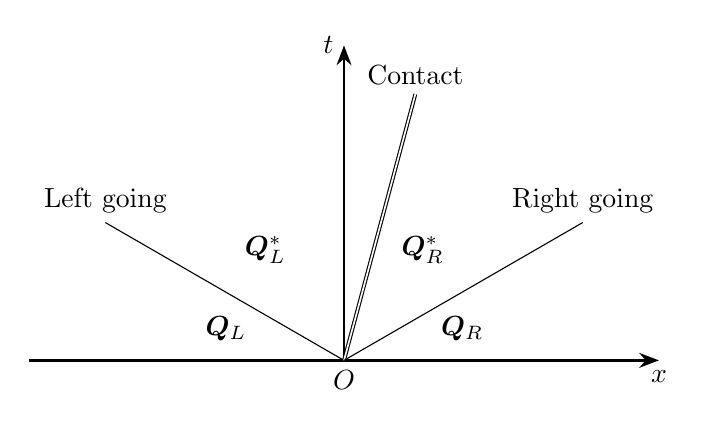
\begin{tikzpicture}
	\draw [line width =1pt,-{Stealth[length=2.5mm]}] (0,0) -- (4,0) node[below]{$x$};
	\draw [line width =1pt] (-4,0) -- (0,0);
	\draw [line width =1pt,-{Stealth[length=2.5mm]}] (0,0) -- (0,4) node[left]{$t$} ;
	\draw (0,0) node [below]{$O$} -- ([turn]-120:3.5) node [above]{Left going};
	\draw [double] (0,0) -- ([turn]165:3.5)   node [above]{Contact};
	\draw (0,0) -- ([turn]120:3.5)  node [above]{Right going};
	\node at (-1.5,0.4) {$\bm{Q}_L$};
	\node at (-1.0,1.4) {$\bm{Q}_L^*$};
	\node at (1.0,1.4) {$\bm{Q}_R^*$};
	\node at (1.5,0.4) {$\bm{Q}_R$};
%	\draw [dashed] (0,0) -- ([turn]135:3.5) node [above]{Right plastic};
%	\draw [dashed] (0,0) -- ([turn]-135:3.5) node [above]{Left plastic} ;
	%\draw [-{Stealth[length=3mm]}] (0,0) -- (2,0);
\end{tikzpicture}
\caption{额鹅鹅鹅}
\end{figure}

\begin{figure}
  \centering
  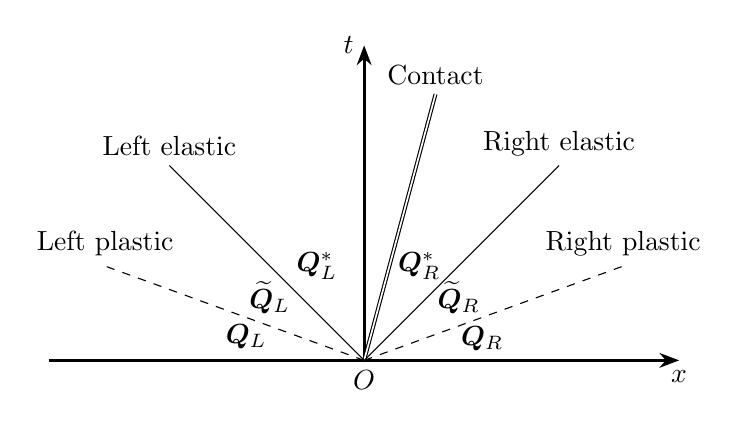
\begin{tikzpicture}
	\draw [line width =1pt,-{Stealth[length=2.5mm]}] (0,0) -- (4,0) node[below]{$x$};
	\draw [line width =1pt] (-4,0) -- (0,0);
	\draw [line width =1pt,-{Stealth[length=2.5mm]}] (0,0) -- (0,4) node[left]{$t$};
	\draw (0,0)[dashed] node [below]{$O$} -- ([turn]-110:3.5) node [above]{Left plastic};
	\draw [double](0,0) -- ([turn]165:3.5)   node [above]{Contact};
	\draw [dashed](0,0) -- ([turn]110:3.5)  node [above]{Right plastic};
	\draw  (0,0) -- ([turn]135:3.5) node [above]{Right elastic};
	\draw  (0,0) -- ([turn]-135:3.5) node [above]{Left elastic} ;
	\node at (-1.5,0.3) {$\bm{Q}_L$};
	\node at (-1.2,0.8) {$\widetilde{\bm{Q}}_L$};
	\node at (-0.6,1.2) {$\bm{Q}_L^*$};
	\node at (0.7,1.2) {$\bm{Q}_R^*$};
	\node at (1.2,0.8) {$\widetilde{\bm{Q}}_R$};
	\node at (1.5,0.28) {$\bm{Q}_R$};
	%\draw [-{Stealth[length=3mm]}] (0,0) -- (2,0);
\end{tikzpicture}
\caption{额鹅鹅鹅}
\end{figure}

Similar to the HLLCE method in Eq.(\ref{eq:HLLCE}), the HLLCEP method is give as follows,
  \begin{equation}\label{eq:HLLCEP}
	\bm{U}^{\text{HLLCEP}}(x,t) = \left\{ \begin{aligned}
		& \bm{U}_L, \hspace{0.3cm} \text{if} \hspace{0.3cm} \frac{x}{t}\le s_L, \\
		& \bm{U}_L^*, \hspace{0.3cm} \text{if} \hspace{0.3cm} s_L\le \frac{x}{t} \le \widetilde{s}_L, \\
		& \widetilde{\bm{U}}_L, \hspace{0.3cm} \text{if} \hspace{0.3cm} \widetilde{s}_L\le \frac{x}{t} \le s^*, \\
		& \widetilde{\bm{U}}_R, \hspace{0.3cm} \text{if} \hspace{0.3cm} s^*\le \frac{x}{t} \le \widetilde{s}_R, \\
		& \bm{U}_R^*, \hspace{0.3cm} \text{if} \hspace{0.3cm} \widetilde{s}_R\le \frac{x}{t} \le s_R,\\
		& \bm{U}_R, \hspace{0.3cm} \text{if} \hspace{0.3cm} \frac{x}{t}\ge s_R, \\
	  \end{aligned}
	\right.
  \end{equation}
  and the corresonding Eulerian and Lagrangian numerical flux are 
 \begin{equation}\label{eq:HLLCEP}
	\bm{F}^{\text{Euler}}(x,t) = \left\{ \begin{aligned}
		& \bm{F}_L, \hspace{0.3cm} \text{if} \hspace{0.3cm} \frac{x}{t}\le s_L, \\
		& \bm{F}_L^*, \hspace{0.3cm} \text{if} \hspace{0.3cm} s_L\le \frac{x}{t} \le \widetilde{s}_L, \\
		& \widetilde{\bm{F}}_L, \hspace{0.3cm} \text{if} \hspace{0.3cm} \widetilde{s}_L\le \frac{x}{t} \le s^*, \\
		& \widetilde{\bm{F}}_R, \hspace{0.3cm} \text{if} \hspace{0.3cm} s^*\le \frac{x}{t} \le \widetilde{s}_R, \\
		& \bm{F}_R^*, \hspace{0.3cm} \text{if} \hspace{0.3cm} \widetilde{s}_R\le \frac{x}{t} \le s_R,\\
		& \bm{F}_R, \hspace{0.3cm} \text{if} \hspace{0.3cm} \frac{x}{t}\ge s_R, \\
	  \end{aligned}
	\right.
  \end{equation}

\begin{equation}
	\bm{F}^{\text{Lag}}(x,t) = \left\{ \begin{aligned}
		& \widetilde{\bm{f}}_L, \hspace{0.3cm} \text{if} \hspace{0.3cm} s_*\ge \frac{x}{t},\\
		& \widetilde{\bm{f}}_R, \hspace{0.3cm} \text{if} \hspace{0.3cm} s^*\le \frac{x}{t}.\\
	  \end{aligned}
	\right.
  \end{equation}

  \subsubsection{ Verifying the plastic waves}
  At first, we need to pre-estimate the deviatoric stresses in regions $\bm{Q}_L^*$ and $\bm{Q}_R^*$ to see if there are yielding happened in the left and right. And to  verify the exists of left and right going plastic waves.  
  
  From the equations in Eq.(\ref{eq:1d}), the density and deviatoric stress can be written in 
  \begin{equation}
	\frac{1}{\rho}\frac{d\rho}{dt}+\frac{\partial u}{\partial x} =0,
  \end{equation}
  and
  \begin{equation}
	\frac{ds_{xx}}{dt}=\frac{4}{3}\mu\frac{\partial u}{\partial x}.
  \end{equation}
So we can get the relation of density and deviatoric stress as
  \begin{equation}
	\frac{ds_{xx}}{dt}=-\frac{4}{3}\mu \frac{1}{\rho}\frac{d\rho}{dt},
\end{equation}
Take an integration from  the region $\bm{Q}_L$ to  the region $\bm{Q}_L^*$, we can get 
\begin{equation}\label{eq:sxxrho}
	s_{xxL}^*=-\frac{4}{3}\mu\text{ln}(\frac{\rho_L^*}{\rho_L})+s_{xxL}.
\end{equation}

If $|s_{xxL}|<\frac{2}{3}Y_0$ and  $|s_{xxL}^*| \ge  \frac{2}{3}Y_0$ there is yielding happened and  plastic wave exists in the left side. On the right side we can take a similar  verifying prcoess.

\subsubsection{ Pre-estimation of  $\rho_L^*$ and  $\rho_R^*$ }
To verify the plastic wave,  we need is to estimate the densities $\rho_L^*$ and $\rho_R^*$. We can pre-estimate them by ignoring the influence of the plastic waves by assuming $\widetilde{\bm{Q}}_L = \bm{Q}_L$ and $\widetilde{\bm{Q}}_R = \bm{Q}_R$. Notice that, the estimated densities is only used  to verify  the yielding process, but not a final result.

According to the Rankine-Hugoniot conditions in Eq.(\ref{eq:RH1}) we have
\begin{equation} \label{eq:rhoLstar}
  \rho_L^* s^*=\rho_L u_L+s_L(\rho_L^*-\rho_L),
\end{equation}
and
\begin{equation}
  \rho_L^* s^{*2}-\sigma^*_L=\rho_L u_L^2-\sigma_L+s_L(\rho_L^* s^*-\rho_L u_L).
\end{equation}
The Cauchy stress can be  estimated as 
\begin{equation}\label{eq:sigmastar}
  \sigma^*_L=\sigma_L + (s_L-u_L)\rho_L u_L +\rho_L^* s^*(s^*-s_L).
\end{equation}

According to the Rankine-Hugoniot conditions in Eq.(\ref{eq:RH2}). Across the contact wave the Cauchy stresses are equavalent. The speed $s^*$  can be  estimated  as
\begin{equation}\label{eq:eva_s}
  s^* = \frac{\sigma_L-\sigma_R+\rho_L u_L(s_L-u_L)-\rho_R u_R(s_R-u_R)}{\rho_L(s_L-u_L)-\rho_R(s_R-u_R)},
\end{equation}
where $s_L$ and $s_R$ are given in the same strategy to Eq.(\ref{eq:sLR}). By Eq.(\ref{eq:rhoLstar}),  we can estimate  the density as
\begin{equation}\label{eq:rhoLs}
  \rho_L^* = \frac{\rho_L(u_L-s_L)}{s^*-s_L}.
\end{equation}


\subsubsection{States of $\widetilde{Q}_L$ and $\widetilde{Q}_R$}
If  there is not  exist a  plastic wave in the left side, $\widetilde{\bm{Q}}_L = \bm{Q}_L$.  Or we need to solve the state behind the plastic wave of $\widetilde{\bm{Q}}_L$.  According to Rankine-Hugoniot relation we can get 
  \begin{align}
	&\widetilde{\rho}_L(\widetilde{u}_L-\widetilde{s}_L) = \rho_L(u_L-\widetilde{s}_L), \label{eq:RHp1}\\
	&\widetilde{\rho}\widetilde{u}_L(\widetilde{u}_L-\widetilde{s}_L) = \rho_Lu_L(u_L-\widetilde{s}_L)+\widetilde{\sigma}_L-\sigma_L,  \label{eq:RHp2}\\
	&\widetilde{\rho}\widetilde{E}_L(\widetilde{u}_L-\widetilde{s}_L) = \rho_LE_L(u_L-\widetilde{s}_L)+\widetilde{\sigma}_L \widetilde{u}_L-\sigma_Lu_L, \label{eq:RHp3}
\end{align}
where yilding happened behind the plastic wave, so the deviatoric stress and density are taken as  
\begin{equation}
  \widetilde{s}_{xxL} =\left\{ \begin{aligned}
	  -\frac{2}{3}Y_0, \hspace{0.3cm} \text{if} \hspace{0.3cm} \rho_L^* > \rho_L,\\
	  \frac{2}{3}Y_0, \hspace{0.3cm} \text{if} \hspace{0.3cm} \rho_L^* < \rho_L,\\
	\end{aligned}\right.
  \end{equation}
  and
\begin{equation}   \widetilde{\rho}_{L} = \left\{ \begin{aligned}
	  & \rho_L \text{exp}\left(\frac{Y_0}{2\mu}+\frac{3 s_{xxL}}{4\mu}\right)  \hspace{0.5cm} \text{if} \hspace{0.3cm} \rho_L^* > \rho_L,\\ 
& \rho_L \text{exp}\left(-\frac{Y_0}{2\mu}+\frac{3 s_{xxL}}{4\mu}\right) 
\hspace{0.3cm} \text{if} \hspace{0.3cm} \rho_L^* < \rho_L.\\ 
  \end{aligned}\right.
 \end{equation}

 The unknowns are the wave speed $\widetilde{s}_L$,  the velocity  $\widetilde{u}_L$, the pressure $\widetilde{p}_L$ and the specific internal energy $\widetilde{E}_L$. In the following, we will give the derivations of   

 From Eq.(\ref{eq:RHp1}) we can get the wave speed
  \begin{equation}
	\widetilde{s}_L = \frac{\widetilde{\rho}_L \widetilde{u}_L-\rho_Lu_L}{\widetilde{\rho}_L-\rho_L},
  \end{equation}
and the relation
\begin{equation}\label{eq:u1_s}
  u_L-\widetilde{s}_L = \frac{(u_L-\widetilde{u}_L)\widetilde{\rho}_L}{\widetilde{\rho}_L-\rho_L}. 
\end{equation}
Substituting Eq.(\ref{eq:RHp1}) into Eq.(\ref{eq:RHp2}), we have 
\begin{equation}\label{eq:rho1}
  \rho_L(\widetilde{u}_L - u_L)(u_L-\widetilde{s}_L) = \widetilde{\sigma}_L -\sigma_L,
\end{equation}
then substituting Eq.(\ref{eq:u1_s}) into it, we can get the following relation
\begin{equation}\label{eq:tu_2}
  -t(\widetilde{u}_L-u_L)^2 = \widetilde{\sigma}_L-\sigma_L,
\end{equation}
where
\begin{equation}
t=\frac{\rho_L \widetilde{\rho}_L}{\widetilde{\rho}_L-\rho_L}.
\end{equation}
Similar to Eq.(\ref{eq:rho1}), Eq.(\ref{eq:RHp2}) can be changed into 
\begin{equation}
  t(u_L-\widetilde{u}_L)(\widetilde{E}_L-E_L) =\widetilde{\sigma}_L\widetilde{u}_L-\sigma_Lu_L,
\end{equation}
and we also know that $E = e+\frac{1}{2}u^2$, then we have 
\begin{equation}\label{eq:e21}
  \widetilde{e}_L-e_L= -\frac{\sigma_L+\widetilde{\sigma}_L}{2t}.
\end{equation}
The EOS (\ref{eq:mie}) can be written as
\begin{equation} \label{eq:eos1}
  e=c_0 p-c_1f(\rho/\rho_0),
\end{equation}
where $c_0=\frac{1}{\rho_0\Gamma_0}$ and $c_1=\frac{a_0^2}{\Gamma_0}$.  

Substituting (\ref{eq:eos1}) and $\sigma=-p +s_{xx}$ into (\ref{eq:e21}), we can get the pressure behind the plastic wave as
\begin{equation}
  \widetilde{p}_L= \frac{2t(c_1f(\widetilde{\rho}_L)+e_L)-(\sigma_L+\widetilde{s}_{xxL})}{2tc_0-1},
\end{equation}
and the Cauchy stress is solved by $\widetilde{\sigma}_L = -\widetilde{p}_L+\widetilde{s}_{xxL}$. Using Eq.(\ref{eq:tu_2}) we can get
\begin{equation}
  (\widetilde{u}_L-u_L)^2 = \frac{\sigma_L-\widetilde{\sigma}_L}{t},
\end{equation}
then the velocity is solved,
\begin{equation}
  \widetilde{\bm{u}}_L= \left\{
  \begin{aligned}
	u_1+\sqrt{\frac{\sigma_L-\widetilde{\sigma}_L}{t}} \hspace{0.2cm} \text{if} \hspace{0.2cm} \rho_R^* >\rho_R,\\
	u_1-\sqrt{\frac{\sigma_L-\widetilde{\sigma}_L}{t}} \hspace{0.2cm} \text{if} \hspace{0.2cm} \rho_R^* <\rho_R.\\
\end{aligned} \right.
\end{equation}
A samilar process is taken to solve the state of $\widetilde{\bm{Q}}_R$.

\subsubsection{Solving the states of $\mathbf{Q}_L^*$ and $\mathbf{Q}_R^*$}
Now we have the states of $\widetilde{\bm{Q}}_L$ and  $\widetilde{\bm{Q}}_R$. Then we can solve the states of   $\bm{Q}_L^*$ and $\bm{Q}_R^*$ easily. 
First we need to pre-estimate the wave speed of $s_L$, $s_R$ and $s^*$ with a same strategy of Eq.(\ref{eq:sLR}) and Eq.(\ref{eq:eva_s}),
\begin{equation}
  s_L = \text{min} (\widetilde{u}_L-\widetilde{c}_L, \widetilde{u}_R-\widetilde{c}_R), \hspace{0.3cm} s_R = \text{max}(\widetilde{u}_L+\widetilde{c}_L, \widetilde{u}_R+\widetilde{c}_R),
	\end{equation}
	\begin{equation}
	  s^* = \frac{\widetilde{\sigma}_L-\widetilde{\sigma}_R+\widetilde{\rho}_L \widetilde{u}_L(s_L-\widetilde{u}_L)-\widetilde{\rho}_R \widetilde{u}_R(s_R-\widetilde{u}_R)}{\widetilde{\rho}_L(s_L-\widetilde{u}_L)-\widetilde{\rho}_R(s_R-\widetilde{u}_R)}.
\end{equation}
Then we can get the density using Eq.(\ref{eq:rhoLs}),
\begin{equation}
  \rho_L^* = \frac{\widetilde{\rho}_L(\widetilde{u}_L-s_L)}{s^*-s_L}, \hspace{0.3cm}  \rho_R^* = \frac{\widetilde{\rho}_R(\widetilde{u}_R-s_R)}{s^*-s_R},
\end{equation}
and the deviatoric stress using Eq.(\ref{eq:sxxrho}),
  \begin{align}
  \hat{s}_{xxL}^* =  -\frac{4}{3}\mu \text{ln}\left( \frac{\rho_L^*}{\rho_L}  \right)+s_{xxL},\\
  \hat{s}_{xxR}^* =  -\frac{4}{3}\mu \text{ln}\left( \frac{\rho_R^*}{\rho_R}  \right)+s_{xxR},\\
\end{align}
then using  the von Mises' yielding condition,
\begin{equation}
  s_{xxL}^* = \Upsilon(\hat{s}_{xxL}^*) , \hspace{0.3cm}  s_{xxR}^* = \Upsilon(\hat{s}_{xxR}^*).
\end{equation}
The Cauchy stresses  are solved by Eq.(\ref{eq:sigmastar}),
\begin{equation}
  \sigma_L^*=\sigma_R^*=\widetilde{\sigma}_L -\widetilde{\rho_L} (s_L-\widetilde{u}_L)(s^*-\widetilde{u}_L).
\end{equation}
So we can get the pressure by $p =s_{xxL}-\sigma$.

\subsection{Summary of HLLCEP}
Here, we present all the procedures of HLLCEP.

Step 1  Estimate $s^*$
\begin{equation*}
  s^* = \frac{\sigma_L-\sigma_R+\rho_L u_L(s_L-u_L)-\rho_R u_R(s_R-u_R)}{\rho_L(s_L-u_L)-\rho_R(s_R-u_R)}.
\end{equation*}

Step 2  Estimate $\rho_L^*$ and $\rho_R^*$
\begin{equation*}
  \rho_L^* = \frac{\rho_L(u_L-s_L)}{s^*-s_L}, \hspace{0.3cm}  \rho_R^* = \frac{\rho_R(u_R-s_R)}{s^*-s_R}.
\end{equation*}

Step 3   Estimate the deviatoric stress
\begin{equation*}
  s_{xxL}^*=-\frac{4}{3}\mu\text{ln}(\frac{\rho_L^*}{\rho_L})+s_{xxL},\hspace{0.2cm}  s_{xxR}^*=-\frac{4}{3}\mu\text{ln}(\frac{\rho_R^*}{\rho_R})+s_{xxR}.
\end{equation*}

Step 4 Solving the state behind the left  plastic wave

\vspace{0.3cm} \hspace{0.4cm}  If $|s_{xxL}| < \frac{2}{3}Y_0 \le |s_{xxL}^*| $, left plastic wave exists, the deviatoric stress, density and pressure  are given as
\begin{equation*}
  \widetilde{s}_{xxL} =\left\{ \begin{aligned}
	  -\frac{2}{3}Y_0, \hspace{0.3cm} \text{if} \hspace{0.3cm} \rho_L^* > \rho_L,\\
	  \frac{2}{3}Y_0, \hspace{0.3cm} \text{if} \hspace{0.3cm} \rho_L^* < \rho_L,\\
	\end{aligned}\right.
	\hspace{0.2cm} \widetilde{\rho}_{L} = \left\{ \begin{aligned}
	  & \rho_L \text{exp}\left(\frac{Y_0}{2\mu}+\frac{3 s_{xxL}}{4\mu}\right)  \hspace{0.5cm} \text{if} \hspace{0.3cm} \rho_L^* > \rho_L,\\ 
& \rho_L \text{exp}\left(-\frac{Y_0}{2\mu}+\frac{3 s_{xxL}}{4\mu}\right) 
\hspace{0.3cm} \text{if} \hspace{0.3cm} \rho_L^* < \rho_L,\\ 
  \end{aligned}\right.
 \end{equation*}
\begin{equation*}
  \widetilde{p}_L= \frac{2t(c_1f(\widetilde{\rho}_L)+e_L)-(\sigma_L+\widetilde{s}_{xxL})}{2tc_0-1}, \hspace{0.3cm} 
t=\frac{\rho_L \widetilde{\rho}_L}{\widetilde{\rho}_L-\rho_L},
\end{equation*}
and the Cauchy stress and velocity are
\begin{equation*}
\widetilde{\sigma}_L = -\widetilde{p}_L+\widetilde{s}_{xxL},
\end{equation*}
\begin{equation*}
  \widetilde{u}_L= \left\{
  \begin{aligned}
	u_L-\sqrt{\frac{\sigma_L-\widetilde{\sigma}_L}{t}} \hspace{0.2cm} \text{if} \hspace{0.2cm} \rho_L^* >\rho_L,\\
	u_L+\sqrt{\frac{\sigma_L-\widetilde{\sigma}_L}{t}} \hspace{0.2cm} \text{if} \hspace{0.2cm} \rho_L^* <\rho_L.\\
\end{aligned} \right.
\end{equation*}
If left plactic wave does not exist,
\begin{equation*}
  \widetilde{\bm{Q}}_L = \bm{Q}_L.
\end{equation*}

Step 5 Solving the state behind the right plastic wave

\vspace{0.3cm} \hspace{0.4cm}  If $|s_{xxR}| < \frac{2}{3}Y_0 \le |s_{xxR}^*| $, right plastic wave exists, the deviatoric stress, density and pressure  are given as
\begin{equation*}
  \widetilde{s}_{xxR} =\left\{ \begin{aligned}
	  -\frac{2}{3}Y_0, \hspace{0.3cm} \text{if} \hspace{0.3cm} \rho_R^* > \rho_R,\\
	  \frac{2}{3}Y_0, \hspace{0.3cm} \text{if} \hspace{0.3cm} \rho_R^* < \rho_R,\\
	\end{aligned}\right.
	\hspace{0.2cm} \widetilde{\rho}_{R} = \left\{ \begin{aligned}
	  & \rho_R \text{exp}\left(\frac{Y_0}{2\mu}+\frac{3 s_{xxR}}{4\mu}\right)  \hspace{0.5cm} \text{if} \hspace{0.3cm} \rho_R^* > \rho_R,\\ 
& \rho_R \text{exp}\left(-\frac{Y_0}{2\mu}+\frac{3 s_{xxR}}{4\mu}\right) 
\hspace{0.3cm} \text{if} \hspace{0.3cm} \rho_R^* < \rho_R,\\ 
  \end{aligned}\right.
 \end{equation*}
\begin{equation*}
  \widetilde{p}_R= \frac{2t(c_1f(\widetilde{\rho}_R)+e_R)-(\sigma_R+\widetilde{s}_{xxR})}{2tc_0-1}, \hspace{0.3cm} 
t=\frac{\rho_R \widetilde{\rho}_R}{\widetilde{\rho}_R-\rho_R},
\end{equation*}
and the Cauchy stress and velocity are
\begin{equation*}
\widetilde{\sigma}_R = -\widetilde{p}_R+\widetilde{s}_{xxR},
\end{equation*}
\begin{equation*}
  \widetilde{u}_R= \left\{
  \begin{aligned}
	u_R+\sqrt{\frac{\sigma_R-\widetilde{\sigma}_R}{t}} \hspace{0.2cm} \text{if} \hspace{0.2cm} \rho_R^* >\rho_R,\\
	u_R-\sqrt{\frac{\sigma_R-\widetilde{\sigma}_R}{t}} \hspace{0.2cm} \text{if} \hspace{0.2cm} \rho_R^* <\rho_R.\\
\end{aligned} \right.
\end{equation*}
If right  plactic wave does not exist,
\begin{equation*}
  \widetilde{\bm{Q}}_R = \bm{Q}_R.
\end{equation*}

Step 6  Solving the wave speeds,
\begin{equation*}
  s_L = \text{min} (\widetilde{u}_L-\widetilde{c}_L, \widetilde{u}_R-\widetilde{c}_R), \hspace{0.3cm} s_R = \text{max}(\widetilde{u}_L+\widetilde{c}_L, \widetilde{u}_R+\widetilde{c}_R),
	\end{equation*}
	\begin{equation*}
	  s^* = \frac{\widetilde{\sigma}_L-\widetilde{\sigma}_R+\widetilde{\rho}_L \widetilde{u}_L(s_L-\widetilde{u}_L)-\widetilde{\rho}_R \widetilde{u}_R(s_R-\widetilde{u}_R)}{\widetilde{\rho}_L(s_L-\widetilde{u}_L)-\widetilde{\rho}_R(s_R-\widetilde{u}_R)}.
\end{equation*}

Step 7  Solving the densities,
\begin{equation*}
  \rho_L^* = \frac{\widetilde{\rho}_L(\widetilde{u}_L-s_L)}{s^*-s_L}, \hspace{0.3cm}  \rho_R^* = \frac{\widetilde{\rho}_R(\widetilde{u}_R-s_R)}{s^*-s_R},
\end{equation*}

Step 8 Solving the deviatoric stresses,
 \begin{align*}
  \hat{s}_{xxL}^* =  -\frac{4}{3}\mu \text{ln}\left( \frac{\rho_L^*}{\rho_L}  \right)+s_{xxL},\\
  \hat{s}_{xxR}^* =  -\frac{4}{3}\mu \text{ln}\left( \frac{\rho_R^*}{\rho_R}  \right)+s_{xxR},\\
\end{align*}
then using  the von Mises' yielding condition,
\begin{equation*}
  s_{xxL}^* = \Upsilon(\hat{s}_{xxL}^*) , \hspace{0.3cm}  s_{xxR}^* = \Upsilon(\hat{s}_{xxR}^*).
\end{equation*}

Step 9  Solving the Cauchy stresses,
\begin{equation*}
  \sigma_L^*=\sigma_R^*=\widetilde{\sigma}_L -\widetilde{\rho_L} (s_L-\widetilde{u}_L)(s^*-\widetilde{u}_L).
\end{equation*}
 Then we can get the pressure by $p =s_{xxL}-\sigma$.

 \section{ A High-order cell-centered Lagrangian scheme for 1D  conservative hydrodynamic equations with Wilkins' model}
 










%
\section*{Acknowledgement} 
This research work was supported by NSFC 11272324, 11272325, NSAF U1530145 and 2016YFA0401200.

\section*{References}

\bibliography{mybibfile}

\newpage
  \appendix
  \renewcommand{\appendixname}{Appendix~}

  \section{The algorithm of the DIP method for solving the convection equations}
\large {\color{black!60!red!80!}}
  \color{black}

\hspace{-0.48cm}
\normalsize
(0) Initiation 
\vspace{0.1cm}

\hspace{0.5cm}
  \scriptsize{\color{black!80}
  \hspace{-0.7cm}
  $
  \left\{
  \begin{array}{l}
	X(i,j)=0\\
	Y(i,j)=0\\
	\end{array}
	\right.
,
\left\{
  \begin{array}{l}
	X_p(i,j)=0\\
	Y_p(i,j)=0\\
	\end{array}
	\right.
,
\left\{
  \begin{array}{l}
	I(i,j)=i\\
	J(i,j)=j\\
	\end{array}
	\right.
,
\left\{
  \begin{array}{l}
	\hat{z}(i,j)=z(i,j)\\
	z_p(i,j)=z(i,j)\\
	\end{array}
	\right.
$

\vspace{0.1cm}
\hspace{-0.48cm}
{ \color{black!60!blue!80}DO}
\color{black!80} $it=1,NT$} {\color{black!60} \hspace{2.3cm} ! Time-Stepping
  \color{black}

  \small \hspace{-0.0cm}
\hspace{-0.18cm}
Solve the decoupled Euler equations (\ref{EulerEquation}) to get $u$, $v$, $\cdots$

\hspace{-0.10cm}
Following is the DIP  algorithm for the convection equations (\ref{Afrac}).
\vspace{0.2cm}

 \normalsize (1) Initial values
  \scriptsize
  { \color{black!80}  
  \vspace{0.1cm}

  \hspace{0.5cm}
$
Mrk(i,j)=0,
S_1(i,j)=0,
S_2(i,j)=0
$
\vspace{0.1cm}

\normalsize \color{black}
(2) Calculate the cell-point
 \scriptsize 
 \vspace{0.1cm}

 \hspace{0.6cm}{\color{black!60!blue!80}DO}
 { \color{black!80} $i=0,NX$}

\hspace{1.1cm} {\color{black!60!blue!80}DO}
{ \color{black!80} $j=0,NY$

\vspace{0.1cm}
 \hspace{1.5cm} $s_x=sign(X(i,j)), s_y=sign(Y(i,j))$

 \hspace{1.5cm}	$\left\{
  \begin{array}{rlr}
u_c(i,j)=&(1-|X|)u(i,j)&+|X|u(i+s_x,j)\\
v_c(i,j)=&(1-|Y|)v(i,j)&+|Y|v(i,j+s_y)\\
	\end{array}
  \right.$}
 \hspace{0.8cm}
   \color{black!60} ! Interpolate velocity according to its location \color{black!80}

 \hspace{1.5cm}	$\left\{
  \begin{array}{l}
	L_x=X(i,j)+u_c(i,j)\Delta t/ \Delta x\\
    L_y=Y(i,j)+v_c(i,j)\Delta t/ \Delta y\\
	\end{array}
	\right.$

%%
 \hspace{1.5cm}	$\left\{
  \begin{array}{l}
	M=i+floor(L_x+0.5)\\
    N=j+floor(L_y+0.5)\\
	\end{array}
  \right.$}
  { \color{black!60} \hspace{3.4cm}
! $(i,j)$ moves to cell $(M,N)$} {\color{black!80}

 \hspace{1.5cm}	$\left\{
  \begin{array}{l}
	X(i,j)=L_x-floor(L_x+0.5)\\
    Y(i,j)=L_y-floor(L_y+0.5)\\
	\end{array}
	\right.$
	{ \color{black!60} \hspace{2.6cm}
! The relative location in $(M,N)$} {\color{black!80}

\vspace{0.1cm}
\hspace{1.5cm} \color{black!60!blue!80} IF
\color{black!70} ($0 \leqslant M \leqslant NX$ and $0 \leqslant N \leqslant NY$)
\color{black!60!blue!80} Then
\color{black!80}
\vspace{0.1cm}

\hspace{2.cm} $Mrk(M,N)=1$

\hspace{2.cm} $S_1(M,N)=S_1(M,N)+1$

\vspace{0.1cm}
\hspace{2.cm}	$\left\{
  \begin{array}{rlr}
    \hat{X}(M,N)=&\{[S_1(M,N)-1]X(M,N)&+X(i,j)\}/S_1(M,N)\\
	\hat{Y}(M,N)=&\{[S_1(M,N)-1]Y(M,N)&+Y(i,j)\}/S_1(M,N)\\
	\hat{z}(M,N)=&\{[S_1(M,N)-1]z(M,N)&+\hat{z}(i,j)\}/S_1(M,N)\\
	\end{array}
  \right.$}
  \hspace{0.0cm}{ \color{black!60} ! Average information} {\color{black!80}}

\vspace{0.1cm}
\hspace{1.5cm} {\color{black!60!blue!80}ENDIF }

\hspace{1cm} {\color{black!60!blue!80}END DO}

\hspace{0.5cm}{ \color{black!60!blue!80}END DO}

\vspace{0.1cm}
\hspace{0.5cm}{\color{black!80}
	$\left\{
  \begin{array}{l}
	X(:,:)=\hat{X}(:,:)\\
	Y(:,:)=\hat{Y}(:,:)\\
	\end{array}
  \right.$}


  \vspace{0.1cm}

\normalsize 
{\color{black}

(3) Calculate the particle-point and update the cell-point$(I,J)$ 
 \scriptsize 

 \vspace{0.1cm}
\hspace{0.6cm}{\color{black!60!blue!80}DO}
{ \color{black!80} $i=0,NX$}

\hspace{1cm}{ \color{black!60!blue!80}DO}
 \color{black!80} $j=0,NY$

\vspace{0.1cm}
 \hspace{1.5cm} $s_x=sign(X_p(i,j)), s_y=sign(Y_p(i,j))$

 \hspace{1.5cm}	$\left\{
  \begin{array}{lll}
u_p(i,j)=&(1-|X_p|)u(I,J)&+|X|u(I+s_x,J)\\
v_p(i,j)=&(1-|Y_p|)v(I,J)&+|Y|v(I,J+s_y)\\
	\end{array}
	\right.$
 \hspace{0.5cm}
  \color{black!60} ! Interpolate velocity according to its position \color{black!80}


 \hspace{1.5cm}	$\left\{
  \begin{array}{l}
	L_x=X_p(i,j)+u_p(i,j)\Delta t/ \Delta x\\
    L_y=Y_p(i,j)+v_p(i,j)\Delta t/ \Delta y\\
	\end{array}
	\right.$

 \hspace{1.5cm}	$\left\{
  \begin{array}{l}
	I(i,j)=I(i,j)+floor(L_x+0.5)\\
    J(i,j)=J(i,j)+floor(L_y+0.5)\\
	\end{array}
	\right.$
  { \color{black!60} \hspace{2.3cm}
! $(i,j)$ moves to cell $(I,J)$} {\color{black!80}

 \hspace{1.5cm}	$\left\{
  \begin{array}{l}
	X_p(i,j)=L_x-floor(L_x+0.5)\\
    Y_p(i,j)=L_y-floor(L_y+0.5)\\
	\end{array}
	\right.$
	{ \color{black!60} \hspace{2.5cm}
! The relative location in $(I,J)$} {\color{black!80}

\vspace{0.1cm}
\hspace{1.5cm} \color{black!60!blue!80} IF
\color{black!70} ($0 \leqslant I \leqslant NX$ and $0 \leqslant J \leqslant NY$)
\color{black!60!blue!80} Then
\color{black!80}

\hspace{2.0cm} $Mrk(I,J)=2$

\hspace{2.0cm} $S_2(I,J)=S_2(I,J)+1$

\hspace{2.0cm}	$\left\{
  \begin{array}{rlr}
	\hat{X}(I,J)=&\{[S_2(I,J)-1]X(I,J)&+X(i,j)\}/S_2(I,J)\\  
	\hat{Y}(I,J)=&\{[S_2(I,J)-1]Y(I,J)&+Y(i,j)\}/S_2(I,J)\\
	\hat{z}(I,J)=&\{[S_2(I,J)-1]z(I,J)&+z_p(i,j)\}/S_2(I,J)\\
	\end{array}
	\right.$
  }
  \hspace{0cm}
  \begin{minipage}{7cm}
	\color{black!60}
! Update cell-point $(I,J)$'s 
 information by averaging 

 \hspace{0.2cm}
all entered particle-points' information
\end{minipage}


 \hspace{9.25cm} 
 \color{black!80}

\vspace{0.1cm}
  \hspace{1.5cm} \color{black!60!blue!80} END IF 

\hspace{1cm} {\color{black!60!blue!80}END DO

\hspace{0.5cm} END DO}

\vspace{0.1cm}

\hspace{0.5cm}{\color{black!80}
	$\left\{
  \begin{array}{l}
	X(:,:)=\hat{X}(:,:)\\
	Y(:,:)=\hat{Y}(:,:)\\
	\end{array}
  \right.$}

  \vspace{0.1cm} 
\normalsize {\color{black}
(4) If there is no cell-point in the cell $(i,j)$, i.e, $Mrk(i,j)=0$
 \scriptsize 

 \vspace{0.1cm} 
\hspace{0.6cm}{\color{black!60!blue!80}DO}
{ \color{black!80} $i=0,NX$}

\hspace{1cm}{ \color{black!60!blue!80}DO}
{ \color{black!80} $j=0,NY$}

\vspace{0.1cm}
\hspace{1.5cm}{ \color{black!60!blue!80}IF}
{ \color{black!80} $Mrk(i,j)=0$}{ \color{black!60!blue!80}then}
{\color{black!80}

\vspace{0.1cm}
\hspace{2cm}  $\left\{
  \begin{array}{l}
	X(i,j)=0\\
	Y(i,j)=0\\
	\end{array}
	\right.$
  }

\hspace{2cm} {\color{black!60!blue!80}IF}
{\color{black!80} $|u(i,j)|\geqslant |v(i,j)|$}{ \color{black!60!blue!80}then}
{ \color{black!60} \hspace{1.4cm} ! Assign a value by interpolating on x-direction}
{\color{black!80}

\small
\hspace{2.5cm} \color{black!80} 
Find two neighboring cell-points located at two sides of $(i,j)$ along x-direction

\scriptsize
\vspace{0.1cm}
\color{black!80}
\hspace{2.5cm} $L=|X(i-il,j)-il)u(i,j)+Y(i-il,j)v(i,j)|$

\hspace{2.5cm} $R=|X(i+ir,j)-ir)u(i,j)+Y(i+ir,j)v(i,j)|$

\hspace{2.5cm} $\hat{z}(i,j)=[R\hat{z}(i-il,j))+L\hat{z}(i+ir,j)]/(R+L)$

\vspace{0.1cm}
\hspace{2cm}{ \color{black!60!blue!80}ELSE}
{\color{black!80}
{ \color{black!60} \hspace{3.9cm} ! Assign a value by interpolating on y-direction}
{\color{black!80}
\vspace{0.1cm}

\hspace{2.5cm} \color{black!80} 
\small
Find two neighboring cell-points located at two sides of $(i,j)$ along y-direction

\vspace{0.1cm}
\scriptsize
\color{black!80}
\hspace{2.5cm} $L=|X(i,j-jl)u(i,j)+(Y(i,j-jl)-jl)v(i,j)|$

\hspace{2.5cm} $R=|X(i,j+jr))u(i,j)+(Y(i,j+jr)-jr)v(i,j)|$

\hspace{2.5cm} $\hat{z}(i,j)=[R\hat{z}(i,j-jl))+L\hat{z}(i,j+jr)]/(R+L)$
}

\vspace{0.1cm}
\hspace{2cm} {\color{black!60!blue!80}END IF

\hspace{1.5cm} END IF}

\hspace{1cm}{ \color{black!60!blue!80}END DO

\hspace{0.5cm} END DO

{\color{black!80}

\vspace{0.1cm}
\hspace{0.5cm} 
\small
Solve the reaction equations (\ref{Rfrac}) to get new $z$ and $z_p$ by using $\hat{z}$

\hspace{0.7cm} 
and $z_p$ to calculate the source terms, respectively.


\vspace{0.1cm}
\scriptsize
\hspace{0.1cm}{ \color{black!60!blue!80}END DO
%
\end{document}
